\documentclass[12pt,]{article}
\usepackage[utf8]{inputenc}
\usepackage[T1]{fontenc}
\usepackage{mathptmx}
\usepackage{geometry}
\usepackage{mathtools}
\usepackage{amsmath}
\usepackage[english]{babel}
\usepackage{graphicx}
\usepackage[os=win]{menukeys}
\usepackage[figurename=Gambar]{caption}
\usepackage{hyperref}
\usepackage{minted}
\usepackage{float}
\usepackage{pdflscape}
\usepackage{pdfpages}
\usepackage[yyyymmdd,hhmmss]{datetime}
\usepackage{tikz}

\newcommand{\ShowOsVersion}{%
	\immediate\write18{\unexpanded{foo=`uname -snrmo` && echo "\\verb+${foo}+" > tmp.tex}}%
	\input{tmp}\immediate\write18{rm tmp.tex}%
}

\newcommand{\ShowTexVersion}{%
	\immediate\write18{\unexpanded{foo=`pdflatex -version | head -n1` && echo "\\verb+${foo}+" > tmp.tex}}%
	\input{tmp}\immediate\write18{rm tmp.tex}%
}

\hypersetup{
	colorlinks=true, %set true if you want colored links
	linktoc=all,     %set to all if you want both sections and subsections linked
	linkcolor=blue,  %choose some color if you want links to stand out
}

\geometry{
	a4paper,
	left=15mm,
	right=10mm,
	top=10mm,
	bottom=10mm,
}

\title{\Large \bf
	Laporan Praktikum Uji Audiometri
}

\author{Achmadi ST MT}
\date{}

\begin{document}
	\maketitle
	\thispagestyle{empty}
	\pagestyle{empty}

	\vspace*{100px}
	\begin{figure}[H]
		\centering
		\includegraphics[width=0.9\linewidth]{result/BestResult}
	\end{figure}

	\vspace*{200px}
	\noindent This report written using:\\
	OS : \ShowOsVersion \\
	TeX : \ShowTexVersion \\
	Update: {\today} at \currenttime\\

	\section{Pendahuluan}

	Dokumen ini adalah laporan teknis yang menjabarkan detil pencapaian dari
	pengembangan unit produk Audiometri yang akan dipasarkan baik kebutuhan medis
	maupun kebutuhan umum.

	\subsection{Requirement}

	Berikut akan dijabarkan acuan kebutuhan (\textit{requirement}) yang terbagi dalam 2 kategori,
	yaitu dari sisi (1) pengguna dan (2) teknis.

	\subsubsection{User}
	Requirement dari sisi pengguna adalah rincian kebutuhan dari sudut pandang pengguna.
	Berikut adalah rangkumannya:
	\begin{itemize}
		\item \textbf{Portabel}. Unit produk harus portabel sehingga tidak terikat secara mandatory
		pada suatu posisi/tempat.
		Parameter portabel mengacu antara lain:
		\begin{itemize}
			\item \textbf{Power source}. Unit harus memiliki sumber tenaga sendiri yang tidak terikat posisi/tempat.
			Dapat berupa battery sekali pakai maupun \textit{rechargeable}.

			\item \textbf{Ukuran}. Unit harus memiliki ukuran volume kecil dan massa yang ringan.
			Ukuran \textit{hand-held} adalah pilihan tepat.

			\item \textbf{Interface}. Unit harus menggunakan \textit{interface} antar muka yang tidak membutuhkan unit
			interface tambahan lain seperti keyboard atau mouse/pointer.
			Dan antar-muka harus terintegrasi dengan unit produk.

		\end{itemize}

		\item \textbf{Storage}. Unit harus memiliki metode atau part untuk menyimpan hasil pengukuran,
		atau mengirimkan hasil itu ke unit lain yang lebih lazim tersedia

		\item \textbf{Intuitif}. Unit harus mengikuti standar produk intuitif sehingga pengguna
		dapat mengoperasikan unit dengan sedikit atau tanpa sama sekali membutuhkan panduan.
	\end{itemize}

	\subsubsection{Teknis}

	Berdasarkan kebutuhan pengguna, maka dapat dirangkum kebutuhan dalam \textit{term} lebih teknis.
	Berikut rangkumannya:
	\begin{itemize}
		\item Unit harus menggunakan daya VDD (3.3 volt) atau VCC (5 volt) dengan konsumsi arus rendah.

		\item Unit harus menggunakan komponen seminimal mungkin agar ukurannya kecil dan ringan.

		\item Unit harus dilengkapi \textit{interface} atau antar-muka pengguna.
		Lebih detil:
		\begin{itemize}
			\item Untuk input cukuplah tombol-tombol push button.
			\item Untuk display cukuplah LCD atau LED indikator.
			\item Jika memungkinkan, jadikan satu input dan display
			dalam bentuk layar sentuh LCD-TFT.
		\end{itemize}
		\item Unit harus memiliki emulasi \textit{filesystem} untuk media peyimpanan seperti
		SDCard, MMC, atau USB-Flashdisk.

		\item Unit harus menyembunyikan semua kompleksitas teknis sehingga mudah digunakan pengguna.
		Jika membutuhkan perangkat lain maka wajib perangkat tersebut sudah lazim tersedia.

	\end{itemize}

	\newpage
	\section{Rancangan}

	\subsection{Overview}
	Dengan memperhatikan \textit{requirement} yang telah dijabarkan, maka dapat dibuat rancangan dari pilihan
	komponen-komponen yang telah ada dan tersedia.
	Berikut bagian utama rancangan:
	\begin{itemize}
		\item CPU menggunakan STM32 Cortex-M4.
		Detil pertimbangan:
		\begin{itemize}
			\item ARM 32-bit Cortex-M4.
			\item Tegangan daya 3.3V.
			\item Ukuran kecil standar paket TQFP.
			\item Tersedia protokol FSMC untuk layar-sentuh LCD-TFT.
			\item Tersedia protokol SPI-FatFs untuk media SDCard/MMC.
			\item Tersedia protokol SPI-I2S untuk Audio PCM.
			\item Tersedia total 144 pin GPIO untuk LED dan tombol.
			\item Harga sangat terjangkau untuk fitur yang tersedia.
		\end{itemize}

		\item Audio DAC (Digital to Analog Converter) MAX98357A.
		Detil pertimbangan:
		\begin{itemize}
			\item Class-D Amplifier.
			\item Tegangan daya 3.3V atau 5V tanpa butuh tegangan negatif.
			\item Protokol PCM 16-bit standar I2S (Inter-Integrated Sound).
			\item Output langsung ke coil/speaker tanpa tambahan amplifier lain.
			\item Tersedia pilihan gain 3dB, 6dB, 9dB (default), 12dB, dan 15dB.
			\item Tersedia fitur Shut-Down untuk \textit{High-Impedance}
			saat tidak menghasilkan output apapun.
		\end{itemize}
	\end{itemize}
	\begin{figure}[H]
		\centering
		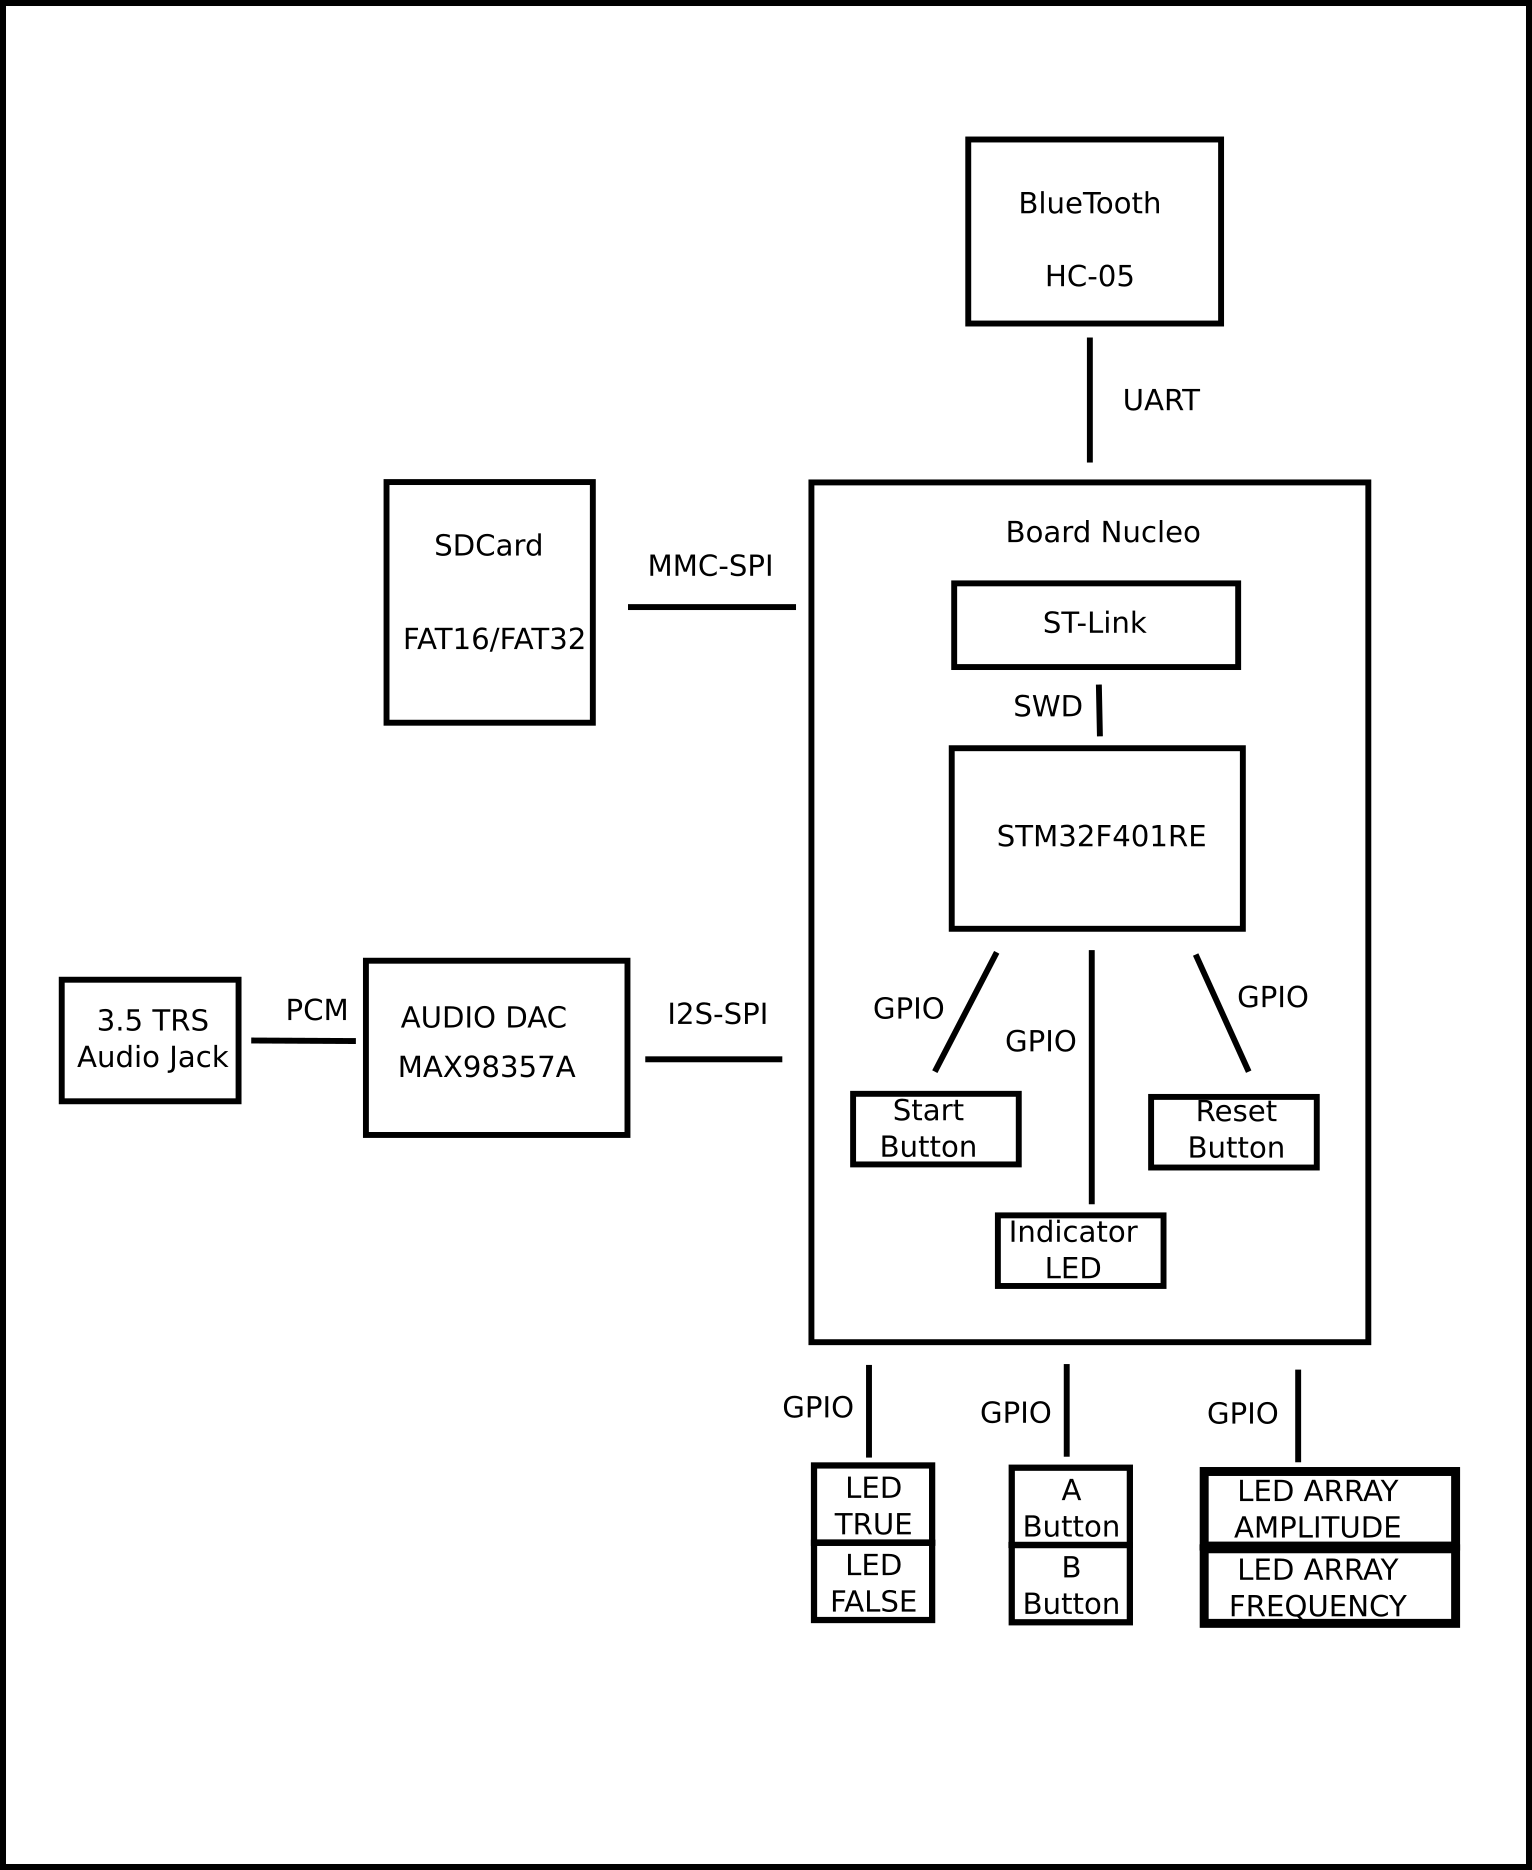
\includegraphics[width=0.6\linewidth]{images/overview}
	\end{figure}

	\newpage
	\subsection{Tone Generator}
	Berikut adalah kelanjutan penjelasan lebih detil tentang bagian tone generator.
	Komponen utama adalah chip STM32 dan Audio DAC MAX98375A.

	\subsubsection{PCM 16-bit}
	PCM (\textit{Pulse-Coded Modulation}) adalah protokol standar untuk bertukar data audio digital.
	Setiap satu frame data PCM terdiri dari 32 bit data untuk channel kanan dan kiri masing-masing 16-bit.
	Jumlah frame mengikuti panjang array buffer yang digunakan.
	Berikut diagram sinyal PCM (dokumentasi chip MAX98357A):
	\begin{figure}[H]
		\centering
		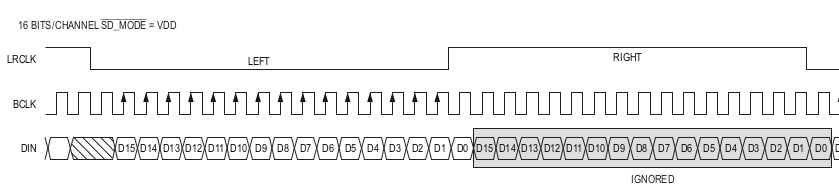
\includegraphics[width=\linewidth]{images/PCM}
	\end{figure}

	Berikut penjelasan 3 sinyal yang dikirim:
	\begin{itemize}
		\item \textbf{LRCLK (Left/Right Clock)}. Sinyal untuk kontrol bagian kanan dan kiri.
		Mengingat chip MAX98357A adalah \textit{mono-amplifier},
		maka posisi sinyal kanan (atau LRCLK berlogika \textit{high}) akan diabaikan.

		\item \textbf{BCLK (Bit Clock)}. Sinyal clock untuk kirim data.
		Chip MAX98357A akan membaca nilai bit data di setiap tepi-naik (\textit{Rising-Edge})
		dari sinyal BCLK.

		\item \textbf{DIN (Data IN)}. Sinyal bit data.
		Satu frame 32-bit Left/Right berasal dari satu variabel elemen dari array buffer.
	\end{itemize}

	Di chip STM32, modulasi PCM dikirim melalui protokol I2S (\textit{Inter-Integrated Sound})
	menggunakan jalur komunikasi SPI (\textit{Serial Peripheral Interface}).
	Secara berurutan, koneksi untuk SPI (MOSI-SCK-NSS) dan untuk I2S (DIN-BCLK-LRCLK).
	Untuk chip MAX98357A tidak dibutuhkan sinyal MCLK (Master Clock).

	\subsubsection{Class-D Amplifier}

	Secara umum, amplifier tipe Class-D adalah jenis amplifier yang tidak mengambil sinyal analog sebagai input.
	Sebaliknya menggunakan sinyal digital PWM (Pulse-Width Modulation) atau PCM (Pulse-Coded Modulation) sebagai input.

	Sinyal input ini kemudian ditumpangkan (dimodulasi) ke PWM frekuensi tinggi dan diamplifikasi sesuai nilai gain.
	Kemudian dengan \textit{low-pass filter}, sinyal dikonversi menjadi lebih analog
	dengan membuang PWM frekuensi tinggi yang "tersisa" di output.
	\begin{figure}[H]
		\centering
		
\includegraphics[width=0.6\linewidth]{images/classD}
	\end{figure}

	\newpage
	Chip MAX98357A menggunakan sinyal dasar \textit{squared} PWM pada frekuensi 300kHz.
	Untuk low-pass filter, digunakan Capasitor 220pF dan Ferrit/Inductor.
	\begin{figure}[H]
		\centering
		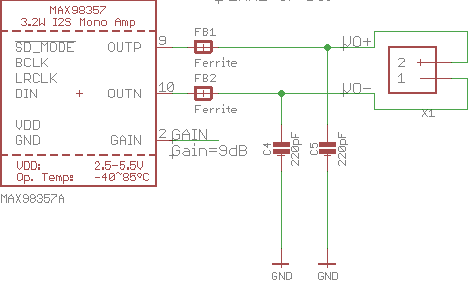
\includegraphics[width=0.6\linewidth]{images/max98357A}
	\end{figure}

	\subsubsection{Programming}
	Berikut adalah penjabaran programming yang digunakan untuk tone generator.
	Penjelasan hanya spesifik untuk protokol I2S tanpa dikaitkan dengan fitur lain.
	Seluruh pustaka/modul programming menggunakan abstraksi dari ChibiOS/RT untuk platform chip STM32F4.

	Untuk mempermudah, maka dibagi dalam bagian-bagian utama.
	Berikut rincian:
	\begin{itemize}
		\item Pengaturan clock untuk peripheral SPI-I2S pada default 96 MHz
		\begin{minted}[frame=lines,fontsize=\footnotesize]{c}
#define STM32_PLLM_VALUE    16
#define STM32_PLLN_VALUE    384
#define STM32_PLLP_VALUE    8
#define STM32_I2SSRC        STM32_I2SSRC_PLLI2S
#define STM32_PLLI2SN_VALUE 288
#define STM32_PLLI2SR_VALUE 3
		\end{minted}

		\item Variabel array buffer.
		Ukuran variabel adalah 16-bit (sesuai ukuran bit PCM).
		Panjang array total harus cukup panjang untuk menghindari
		noise akibat zero-padding yang tidak tercapai.
		\begin{minted}[frame=lines,fontsize=\footnotesize]{c}
uint16_t i2s_tx_buf[512*16];
		\end{minted}

		\item Variabel Driver I2S.
		Disini dimasukkan variabel array buffer.
		Juga didefinisikan ukuran buffer yang akan di \textit{play-loop}.
		Ukuran buffer play ini harus lebih kecil daripada total array buffer
		dan akan mempengaruhi frekuensi tone yang dihasilkan.
		Ukuran buffer play default adalah 512.
		Frekuensi BCLK diatur pada 16kHz.
		\begin{minted}[frame=lines,fontsize=\footnotesize]{c}
I2SConfig i2scfg = {
	i2s_tx_buf,
	NULL,
	512,
	NULL,
	0,
	16,
};
		\end{minted}

		\newpage
		\item Mengatur semua nilai array ke 0.
		Model matematis:
		\[ Y(i) = 0, \text{ for } 0 \leq i < 512 \]
		Dan model \textit{array-loop}:
		\begin{minted}[frame=lines,fontsize=\footnotesize]{c}
for(i=0;i<512;i++){
	i2s_tx_buf[i] = 0;
}
		\end{minted}

		\item Mengatur sine tone.
		Fungsi ini akan dimodifikasi dan disesuaikan hingga mendapatkan
		tone yang paling bersih pada frekuensi yang lebih tinggi
		dari frekuensi yang diinginkan.
		Model matematis:
		\[ Y(i) = sin(2\pi f \frac{i}{512}), \text{ for } 0 \leq i < 512 \]
		Dan model array-loop:
		\begin{minted}[frame=lines,fontsize=\footnotesize]{c}
for(i=0;i<512;i++){
	i2s_tx_buf[i] = sin((double) freq*i*2*(M_PI/512));
}
		\end{minted}

		\item \textit{Playing} sine array dalam \textit{looping}
		terus-menerus dalam rentang durasi (dalam detik).
		I2S menggunakan SPI channel 2 sehingga menggunakan driver I2SD2.
		\begin{minted}[frame=lines,fontsize=\footnotesize]{c}
i2sStart(&I2SD2, &i2scfg);
i2sStartExchange(&I2SD2);

chThdSleepMilliseconds(duration*1000);

i2sStopExchange(&I2SD2);
i2sStop(&I2SD2);
		\end{minted}
	\end{itemize}

	Seluruh \textit{source-code} tersedia di repository github milik Lab Vibrastik.
	Beberapa file penting untuk dievaluasi terkait tone generator:

	\begin{itemize}
		\item \textbf{mcuconf.h}. Berisi pengaturan clock untuk STM32 dan fitur I2S.\\
		\url{https://github.com/VibrasticLab/pikoakustik/blob/master/nucleo401/mcuconf.h}

		\item \textbf{ht\_audio.h}. Berisi makro/definisi untuk fitur tone generator.\\
		\url{https://github.com/VibrasticLab/pikoakustik/blob/master/nucleo401/ht_audio.h}

		\item \textbf{ht\_audio.c}. Berisi referensi dan implementasi proses tone generator.\\
		\url{https://github.com/VibrasticLab/pikoakustik/blob/master/nucleo401/ht_audio.c}
	\end{itemize}

	\newpage
	\section{Pengujian dan Hasil}

	\subsection{Requirement}
	\textit{Prototype} unit tone generator pada tahapan pengembangan ini sudah dapat
	menghasilkan tone melalui headphone via jack 3.5mm tipe TRS (\textit{Tip-Round-Sleeve}).

	Namun untuk memastikan kualitas tone yang dihasilkan,
	diperlukan pengujian lebih jauh terkait poin-poin seperti berikut:
	\begin{enumerate}
		\item Apakah tone yang dihasilkan hanya satu frekuensi dan bersih dari frekuensi derau?
		\item Bagaimana pergeseran frekuensi terhadap perubahan clock maupun panjang array buffer?
		\item Bagaimana pergeseran amplitudo terhadap maximum SPL di frekuensi yang diinginkan?
		\item Bagaimana hubungan pergeseran frekuensi terhadap amplitudo frekuensi yang diinginkan?
		\item Apakah array buffer yang dihasilkan sudah sesuai dengan array untuk channel mono?
		\item Apakah masih menghasilkan \textit{audio-pop} saat menghasilkan tone?
	\end{enumerate}

	Untuk menguji dan memperbaiki (modifikasi), digunakan alat bantu \textit{Audio Analyzer} dalam
	produk manekin KEMAR buatan GRAS.

	Secara umum, skema pengujian \textit{tone generator}.

	\begin{figure}[H]
		\centering
		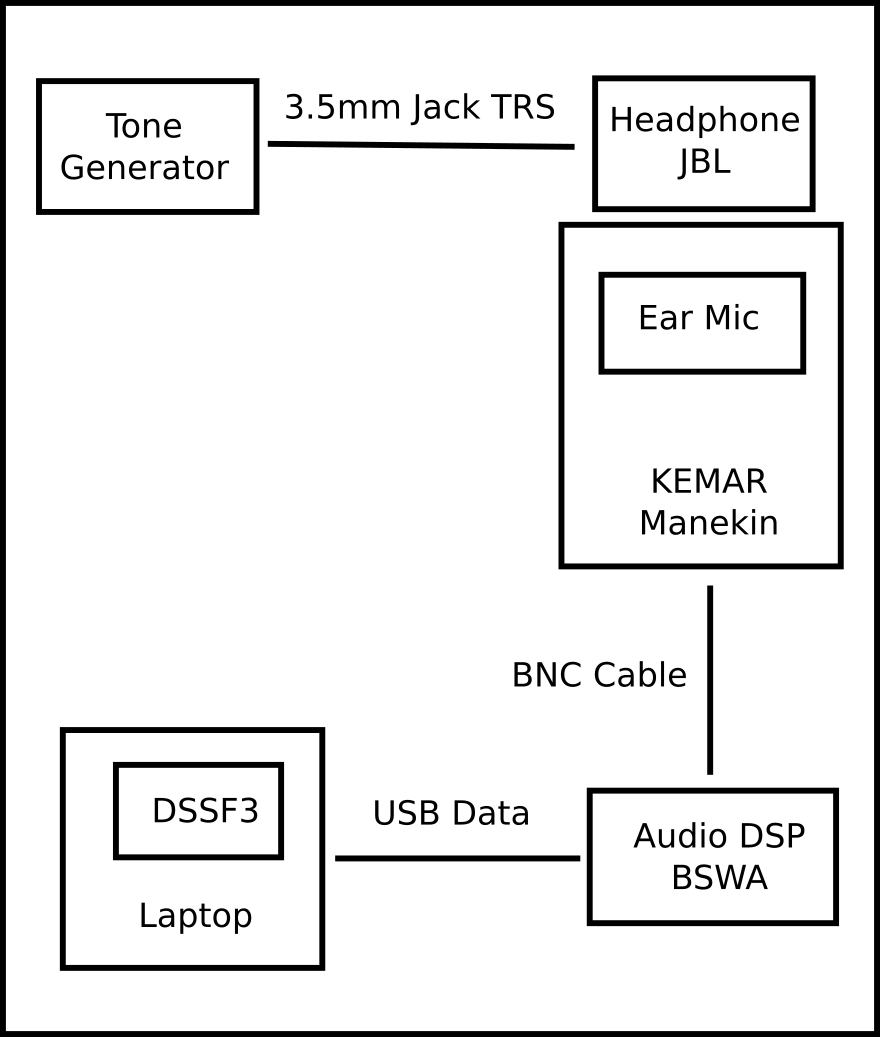
\includegraphics[width=0.5\linewidth]{images/kemar}
	\end{figure}

	\subsection{Persiapan}

	Sebagai dokumentasi berikut dijabarkan langkah-langkah setup manekin KEMAR dan Audio Analyzer.

	\begin{itemize}
		\item Posisikan manekin KEMAR di atas alas datar (disini digunakan kardus).
		\item Atur Posisi hadap kepala di 0 derajat.
		\item Siapkan daun telinga karet

		\newpage
		\begin{figure}[H]
			\centering
			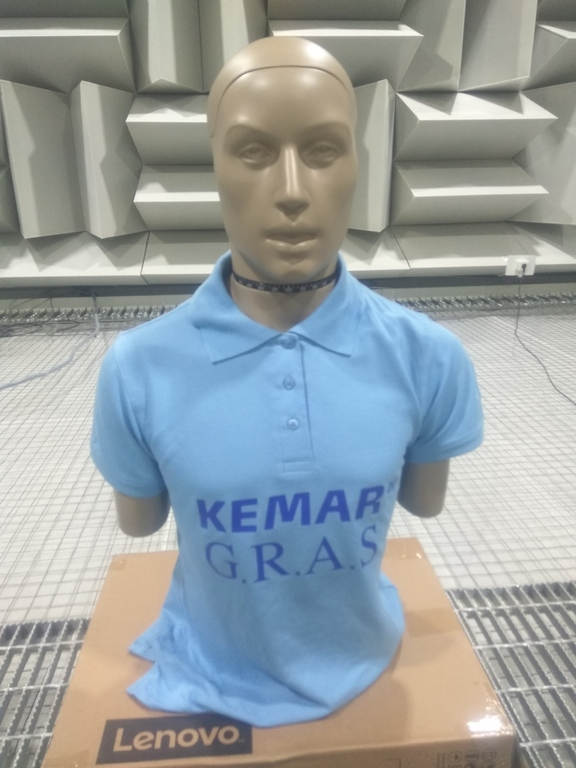
\includegraphics[width=0.3\linewidth]{day_1/manekin0}
			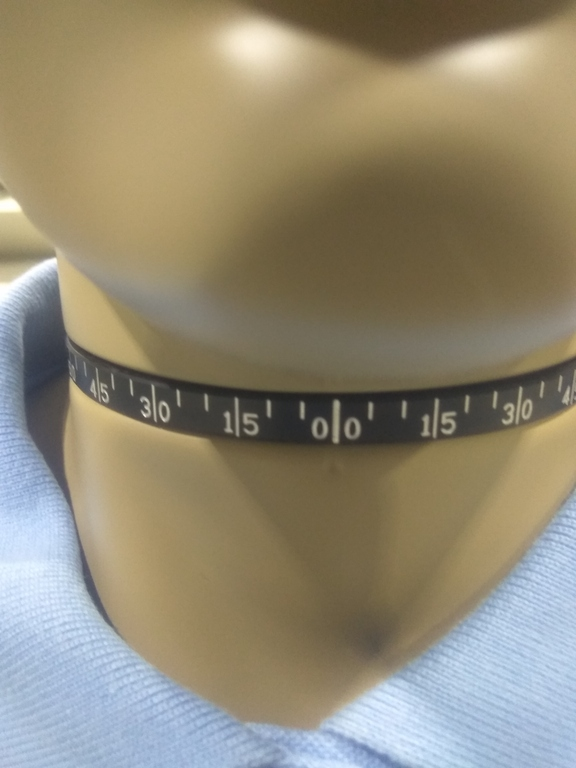
\includegraphics[width=0.3\linewidth]{day_1/manekin1}
			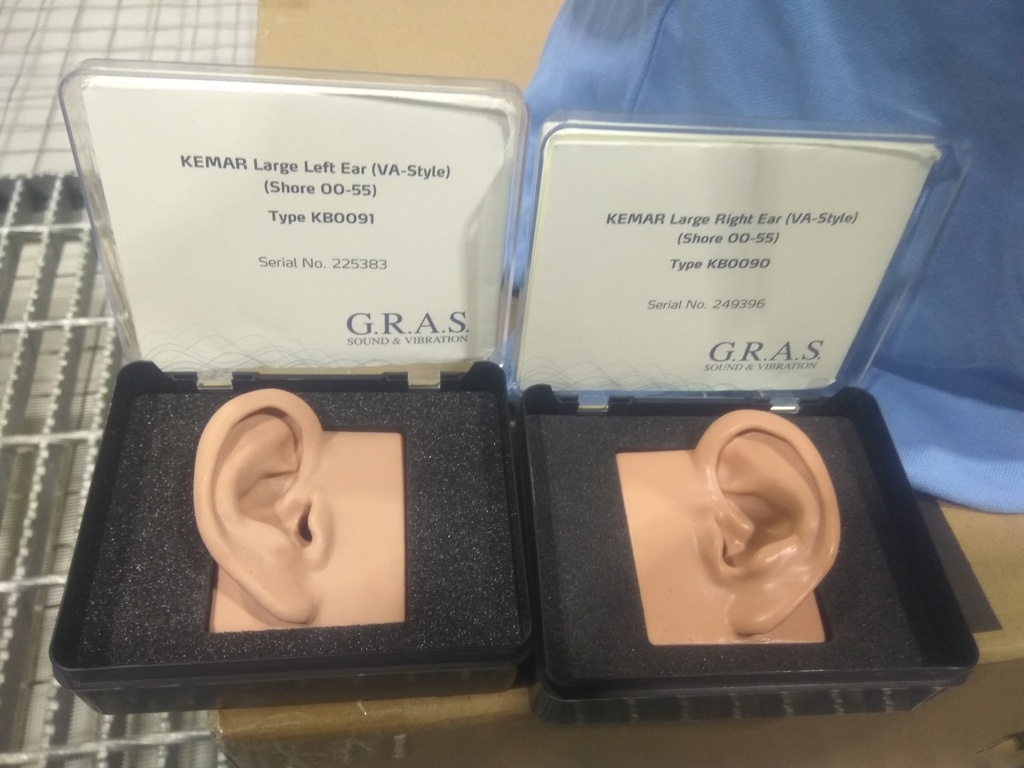
\includegraphics[width=0.3\linewidth]{day_1/earleaf0}
		\end{figure}

		\item Sambungkan Output Mic ke Audio DSP melalui kabel BNC
		\begin{figure}[H]
			\centering
			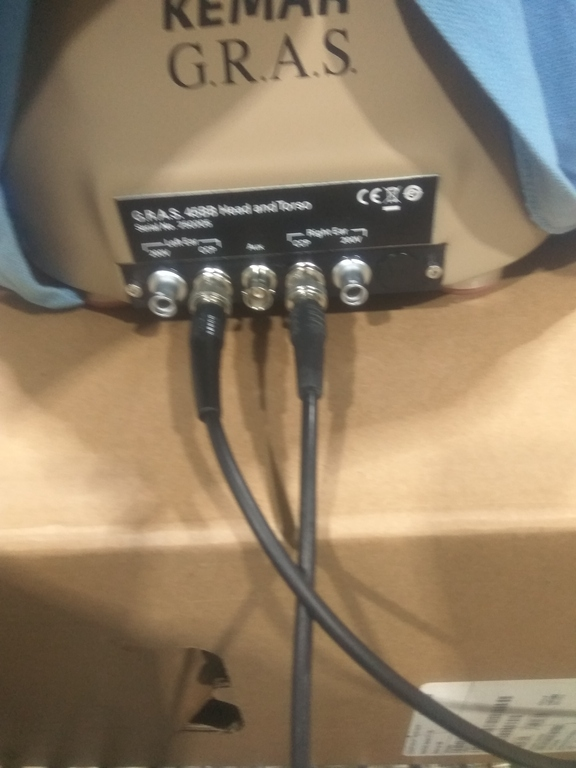
\includegraphics[width=0.3\linewidth]{day_1/wiring0}
			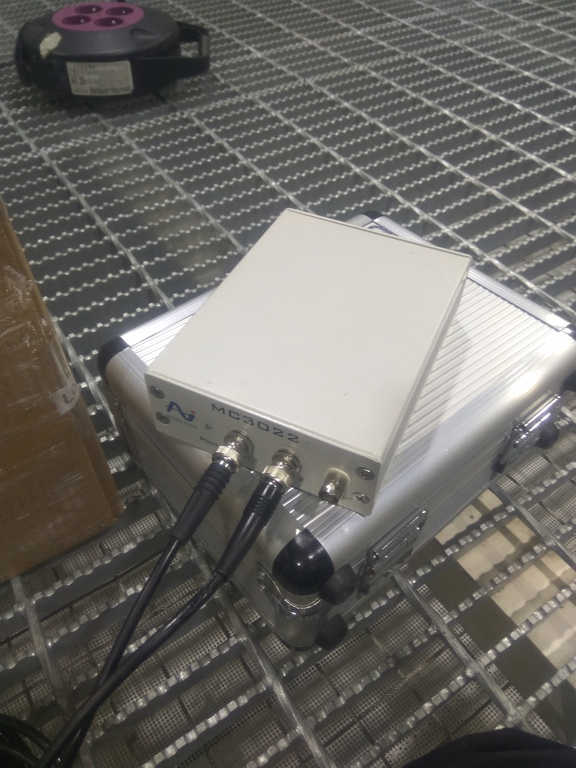
\includegraphics[width=0.3\linewidth]{day_1/wiring1}
		\end{figure}

		\item Sambungkan Audio DSP ke laptop dan jalankan program DSSF3.
		Buka tab \textbf{FFT Analyzer} dan klik tombol \textbf{Calibration}.

		\item Kalibrasi menggunakan standar tone kalibrator yang satu paket dengan KEMAR
		Acuan standar kalibrasi pada SPL 114 dB dan frekuensi 250 Hz.
		Kalibrasi dilakukan pada kedua telinga.
		\begin{figure}[H]
			\centering
			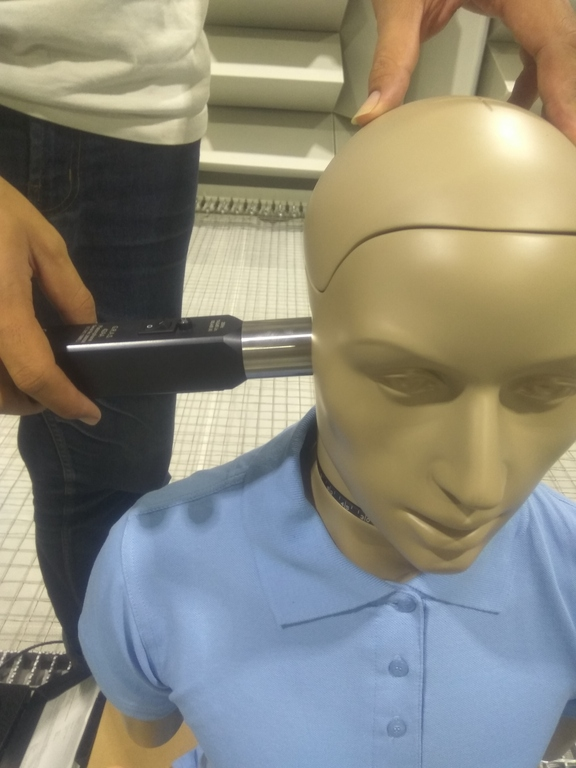
\includegraphics[width=0.3\linewidth]{day_1/kalib0}
			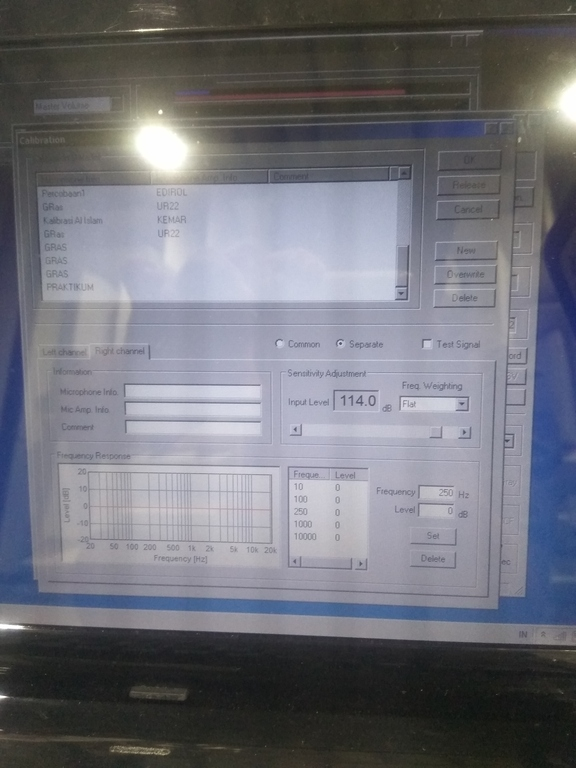
\includegraphics[width=0.3\linewidth]{day_1/kalib1}
			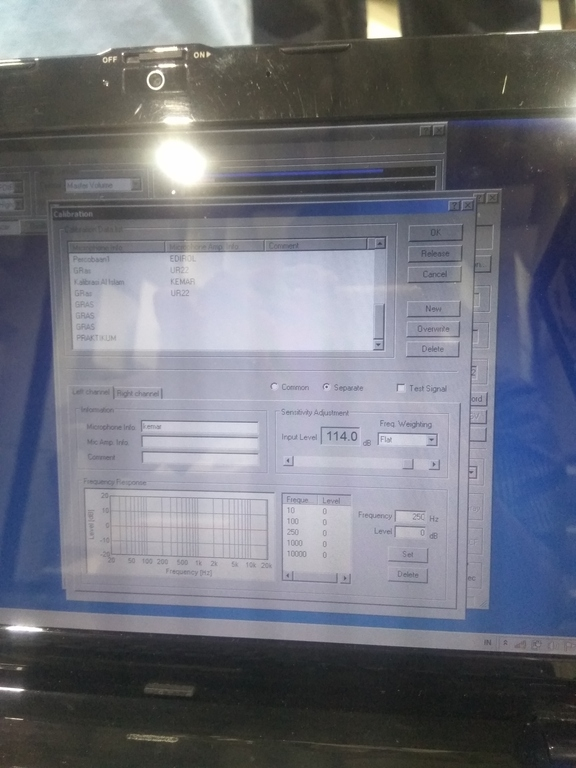
\includegraphics[width=0.3\linewidth]{day_1/kalib2}
		\end{figure}

		\newpage
		\item Pasang daun telinga karet
		\begin{figure}[H]
			\centering
			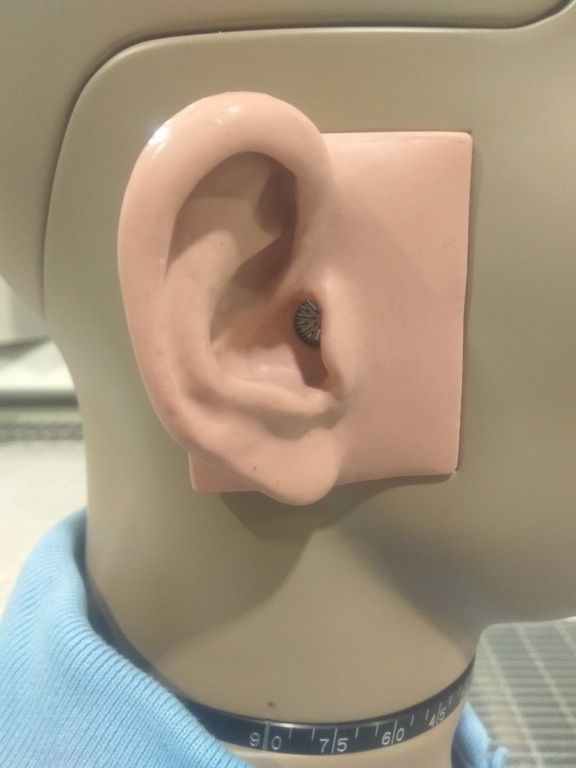
\includegraphics[width=0.3\linewidth]{day_1/earleaf1}
			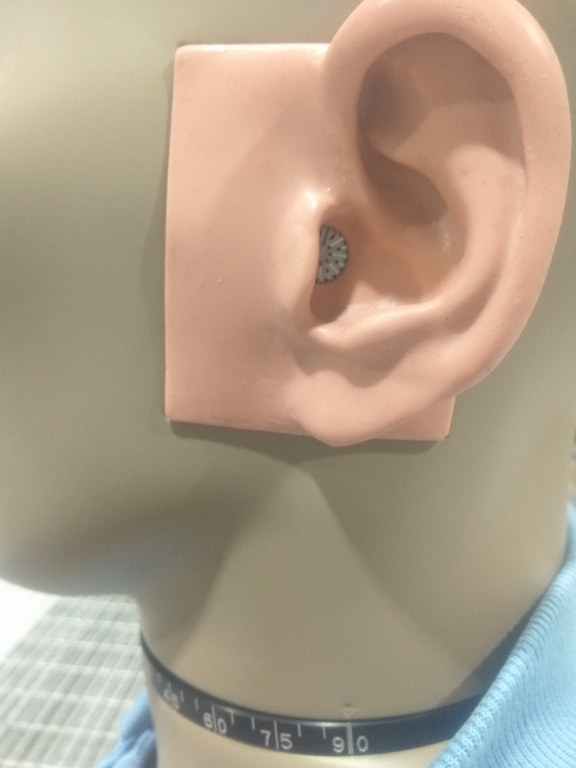
\includegraphics[width=0.3\linewidth]{day_1/earleaf2}
		\end{figure}

		\item Pasang headphone
		\begin{figure}[H]
			\centering
			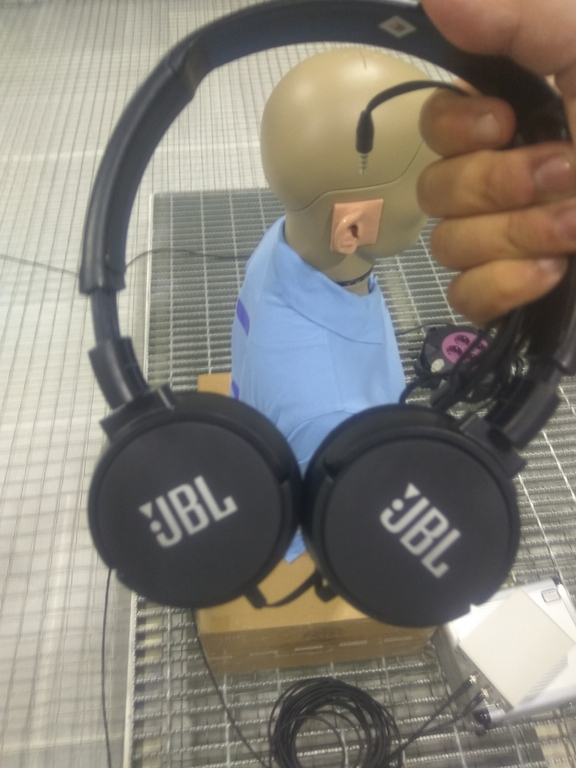
\includegraphics[width=0.3\linewidth]{day_1/phone0}
			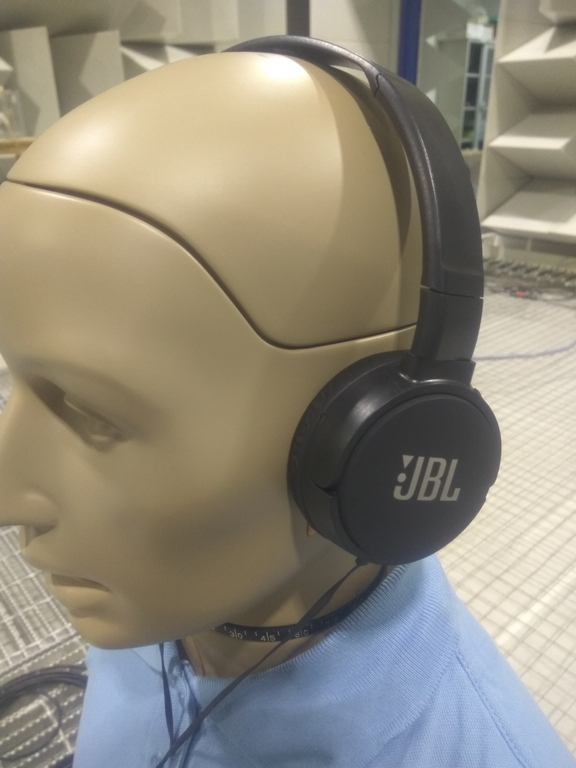
\includegraphics[width=0.3\linewidth]{day_1/phone1}
			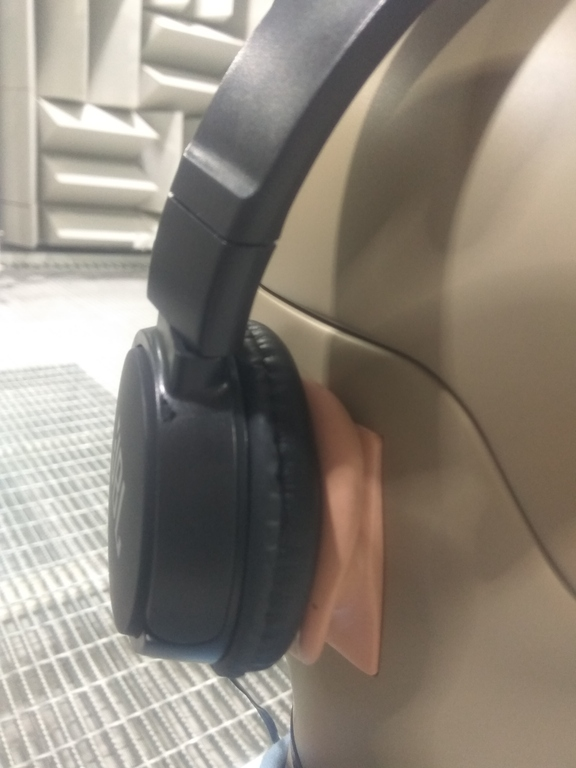
\includegraphics[width=0.3\linewidth]{day_1/phone2}
		\end{figure}

		\item Sambungkan headphone ke tone generator.
		Sebagai uji awal, dilakukan uji respon FFT untuk melihat apakah setup sudah bekerja.

		\begin{figure}[H]
			\centering
			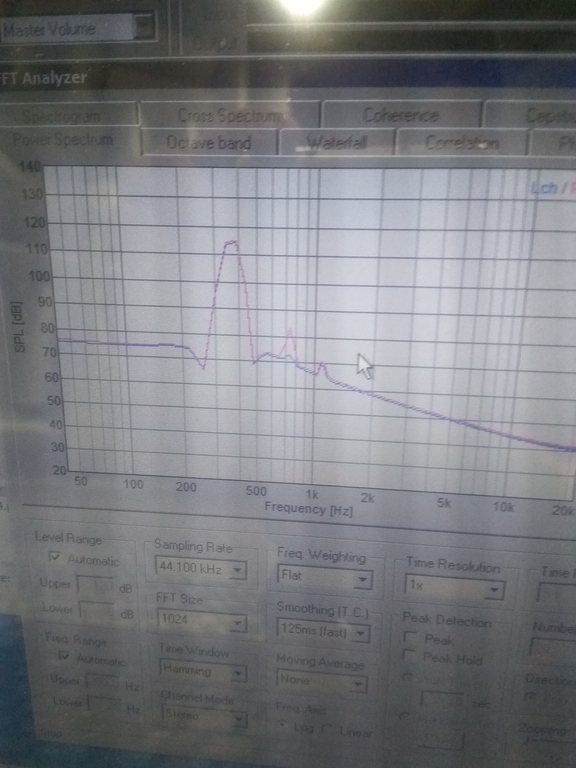
\includegraphics[width=0.3\linewidth]{day_1/test0}
			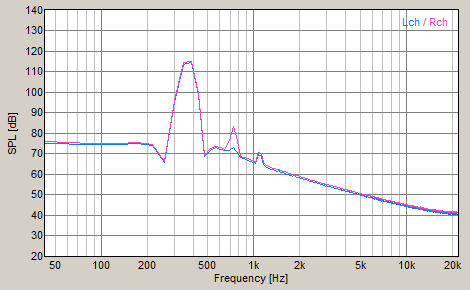
\includegraphics[width=0.6\linewidth]{day_1/test1}
		\end{figure}
	\end{itemize}

	\subsection{Uji Model/Persamaan Array}

	Berikut adalah hasil uji model atau persamaan yang menghasilkan array untuk dikirim sebagai PCM.

	\subsubsection{Model konstanta array}
	Array ini menggunakan konstanta array dengan ukuran 256.
	Nilai konstanta array ini dapat dilihat di file \textbf{ht\_audio.c} pada variabel \textbf{sine\_table}:\\
	\url{https://github.com/VibrasticLab/pikoakustik/blob/master/nucleo401/ht_audio.c}\\
	Ini adalah model yang pertama diuji karena tersedia di dokumentasi pustaka ChibiOS/RT.
	Berikut bentuk plot nilai array dan respon FFT nya.

	\begin{figure}[H]
		\centering
		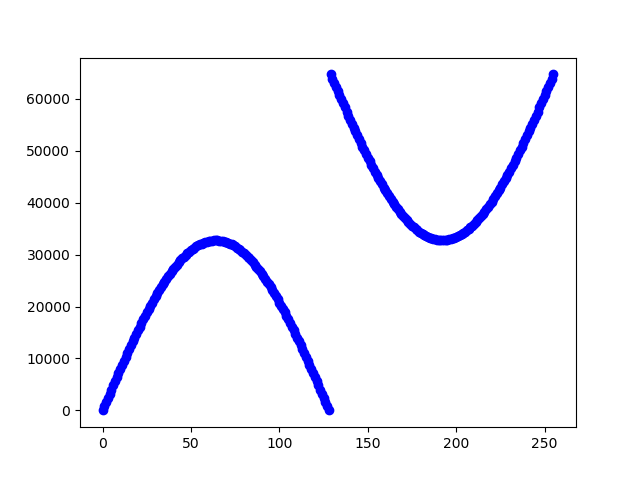
\includegraphics[width=0.45\linewidth]{result/day_1/rev_sine_table}
		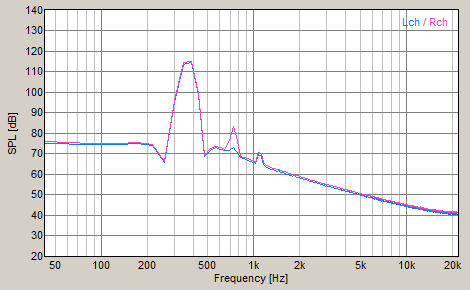
\includegraphics[width=0.45\linewidth]{result/day_1/tableMax256}
	\end{figure}

	Masih terlihat jelas ada frekuensi tambahan (derau) di atas frekuensi yang diinginkan.

	\subsubsection{Model persamaan reversed-sine}
	Berdasarkan hasil sebelumnya, maka dibuat persamaan array untuk menghasilkan pola sinus terbalik
	seperti pada konstanta array (ukuran 256) pada uji sebelumnya.
	Model matematis.
	\[
	Y(i) =
	\begin{cases}
	A sin(\pi \frac{i}{127}), \text{ if } 0 \leq i < 127\\
	A(2-sin(\pi \frac{i}{127})), \text{ if } 127 \leq i < 256\\
	\end{cases}
	 \]
	 dengan A adalah nilai maksimal variabel \textit{signed 16-bit} yaitu 32767.
	 Dalam bentuk array loop:
	 \begin{minted}[frame=lines,fontsize=\footnotesize]{c}
for(i=0;i<127;i++){
	i2s_tx_buf[i] = 32767*sin(3.141592653589793*((double)i/(double)127));
	i2s_tx_buf[127+i] = 32767*(2-sin(3.141592653589793*((double)i/(double)127)));
}
	 \end{minted}
	 Hasilnya tidak lebih bersih dari sebelumnya. Masih muncul derau cukup banyak.
	 \begin{figure}[H]
	 	\centering
	 	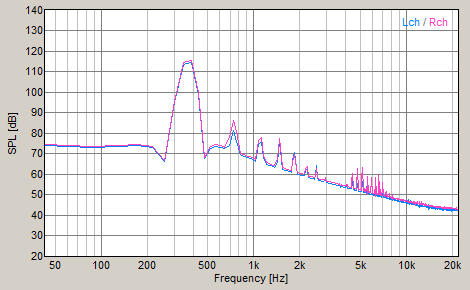
\includegraphics[width=0.45\linewidth]{result/day_1/halfMax256}
	 \end{figure}

 	 \newpage
 	 \subsubsection{Model persamaan sine}
 	 Dengan melihat hasil sebelumnya yang kurang memuaskan, dilakukan uji untuk model sinus.
 	 Model matematis:
 	 \[ Y(i) = A sin(2\pi f \frac{i}{B}), \text{ for } 0 \leq i < B \]
 	 dengan A adalah nilai maksimal variabel \textit{signed 16-bit} yaitu 32767
 	 dan B adalah ukuran buffer array.
 	 Model array loop:
 	 \begin{minted}[frame=lines,fontsize=\footnotesize]{c}
for(i=0;i<I2S_BUFF_SIZE;i++){
	i2s_tx_buf[i] = 32767*sin((double) i*2*(M_PI/I2S_BUFF_SIZE));
}
 	 \end{minted}
 	 Berikut hasil dengan variasi panjang array:
 	 \begin{itemize}
 	 	\item 256
 	 	\begin{figure}[H]
 	 		\centering
 	 		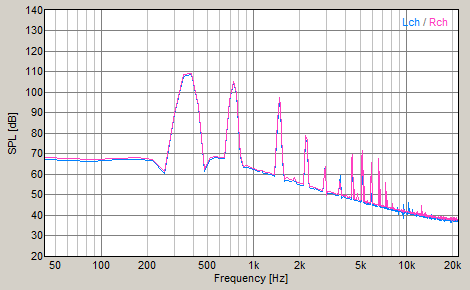
\includegraphics[width=0.45\linewidth]{result/day_1/max256}
 	 	\end{figure}

  		\item 512
  		\begin{figure}[H]
  			\centering
  			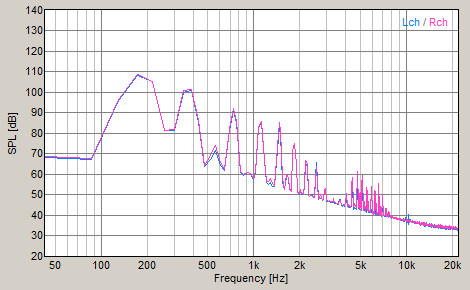
\includegraphics[width=0.45\linewidth]{result/day_1/max512}
  		\end{figure}

  		\item 1024
  		\begin{figure}[H]
  			\centering
  			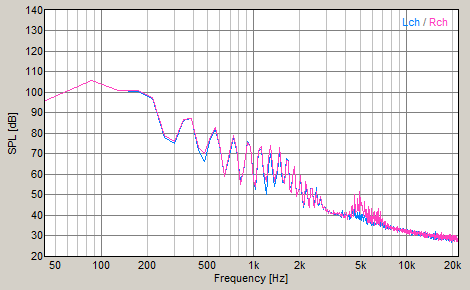
\includegraphics[width=0.45\linewidth]{result/day_1/max1024}
  		\end{figure}
 	 \end{itemize}

  	\newpage
  	\subsubsection{Variasi Clock I2S}
  	Melihat hasil sebelumnya yang jauh dari harapan, maka dilakukan modifikasi
  	pengaturan nilai clock untuk peripheral I2S.
  	Pengaturan ini dapat dilihat di file \textbf{mcuconf.c} pada makro I2SN dan I2SR:\\
  	\url{https://github.com/VibrasticLab/pikoakustik/blob/master/nucleo401/mcuconf.c}\\
  	Model yang digunakan tetap pada model array sebelumnya dengan panjang array 256.
  	Berikut hasilnya:
  	\begin{itemize}
  		\item Variasi 48MHz
  		\begin{minted}[frame=lines,fontsize=\footnotesize]{c}
#define STM32_PLLI2SN_VALUE 288
#define STM32_PLLI2SR_VALUE 6
  		\end{minted}
  		\begin{figure}[H]
  			\centering
  			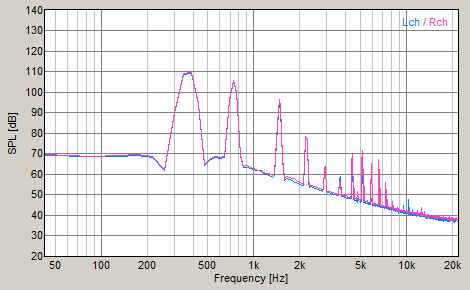
\includegraphics[width=0.45\linewidth]{result/day_2/sine_clk48}
  		\end{figure}

  		\item Variasi 72MHz
  		\begin{minted}[frame=lines,fontsize=\footnotesize]{c}
#define STM32_PLLI2SN_VALUE 288
#define STM32_PLLI2SR_VALUE 4
  		\end{minted}
  		\begin{figure}[H]
  			\centering
  			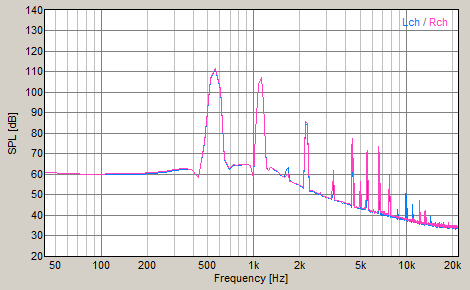
\includegraphics[width=0.45\linewidth]{result/day_2/sine_clk72}
  		\end{figure}

  		\item Variasi 96MHz
  		\begin{minted}[frame=lines,fontsize=\footnotesize]{c}
#define STM32_PLLI2SN_VALUE 288
#define STM32_PLLI2SR_VALUE 3
  		\end{minted}
  		\begin{figure}[H]
  			\centering
  			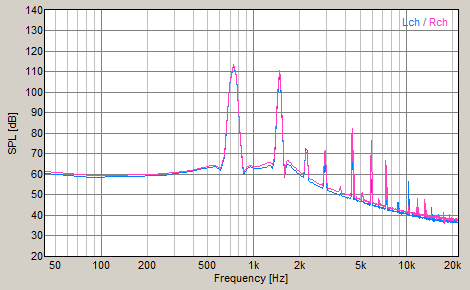
\includegraphics[width=0.45\linewidth]{result/day_2/sine_clk96}
  		\end{figure}
  	\end{itemize}

  	\newpage
  	\subsubsection{Model Sinus Signed 16-bit}
  	Model sinus berikut adalah sinus dimana nilai negatif ditempatkan
  	pada posisi overflow variable signed 16-bit (65535 hingga 32767).
  	Bentuk model matematis:
  	\[
  	Y(i) =
  	\begin{cases}
  	A sin(2 \pi \frac{i}{512}), \text{ if } Y \geq 0, \text{ for } 0 \leq i < 512\\
  	A sin(2 \pi \frac{i}{512})+65535, \text{ if } Y < 0, \text{ for } 0 \leq i < 512
  	\end{cases}
  	\]
  	dengan A adalah nilai maksimal variabel \textit{signed 16-bit} yaitu 32767.
  	Model array-loop:
  	\begin{minted}[frame=lines,fontsize=\footnotesize]{c}
for(i=0;i<512;i++){
  	ysin = 32767*sin(2*3.141592653589793*((double)i/(double)512));
  	if(ysin >= 0){ i2s_tx_buf[i]=ysin; }
  	if(ysin <0  ){ i2s_tx_buf[i]=ysin+65535; }
}
  	\end{minted}
  	\begin{figure}[H]
  		\centering
  		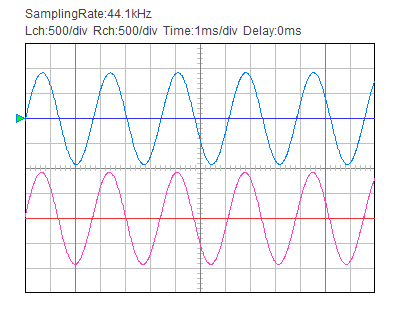
\includegraphics[width=0.45\linewidth]{result/day_4/newsine400}
  		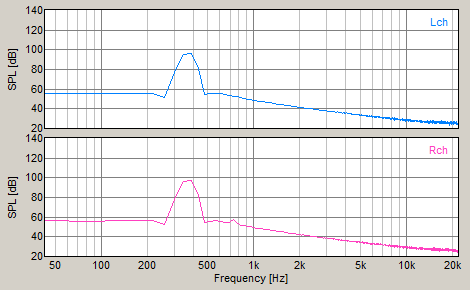
\includegraphics[width=0.45\linewidth]{result/day_4/newsine400fft}
  	\end{figure}

  	Ini adalah model sinus yang paling bersih hingga saat ini
  	dan model ini yang menjadi standar model array sinus untuk pengembangan selanjutnya.
  	Sebagai tambahan konfirmasi, maka hasil ini juga di uji menggunakan osiloskop 200kHz.
  	\begin{figure}[H]
  		\centering
  		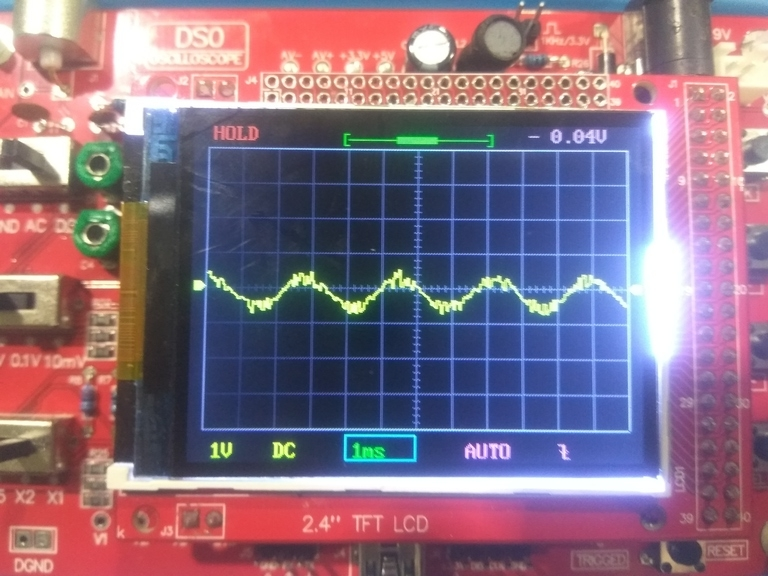
\includegraphics[width=0.45\linewidth]{result/day_4/goodsine}
  	\end{figure}
  	Dapat terlihat masih belum sepenuhnya \textit{smooth},
  	masih ada sisa sinyal squared pada frekuensi tinggi,
  	namun karena osiloskop ini bekerja pada 200kHz,
  	maka kemungkinan tidak tertangkap pada Audio Analyzer yang diatur pada rentang 44100Hz.

  	\newpage
  	Sebagai tambahan informasi, berikut tambahan \textit{screen-shot} hasil tersebut:
  	\begin{figure}[H]
  		\centering
  		\includegraphics[width=0.9\linewidth]{result/day_4/BestResult}
  	\end{figure}

  	\subsubsection{Pergeseran Frekuensi}
  	Pengujian selanjutnya adalah bagaimana respon frekuensi terhadap perubahan panjang array.
  	Model matematis:
  	\[ B = 512/F \]
  	\[
  	Y(i) =
  	\begin{cases}
  	A sin(2 \pi \frac{i}{B}), \text{ if } Y \geq 0, \text{ for } 0 \leq i < B\\
  	A sin(2 \pi \frac{i}{B})+65535, \text{ if } Y < 0, \text{ for } 0 \leq i < B
  	\end{cases}
  	\]
  	dengan A adalah nilai maksimal variabel \textit{signed 16-bit} yaitu 32767
  	dan F adalah skala untuk memodifikasi panjang array buffer.
  	Model array-loop:
  	\begin{minted}[frame=lines,fontsize=\footnotesize]{c}
buffsize = (uint16_t) 512/freq;
for(i=0;i<buffsize;i++){
	ysin = 32767*sin(2*3.141592653589793*((double)i/(double)buffsize));
	if(ysin >= 0){ i2s_tx_buf[i]=ysin; }
	if(ysin <0  ){ i2s_tx_buf[i]=ysin+65535; }
}
i2scfg.size = buffsize;
  	\end{minted}
  	Untuk mendapatkan nilai frekuensi dan spl, digunakan perhitungan Left/2+Right/2 (sesuai dokumentasi MAX98357A).
  	\[ f = \frac{f_{left} + f_{right}}{2}  \]
  	\[ P = \frac{P_{left} + P_{right}}{2}  \]
  	Ekstraksi data CSV dan nilai frekuensi/SPL menggunakan skrip python semisal berikut:\\
  	\url{https://github.com/VibrasticLab/pikoakustik/blob/master/nucleo401/doc/itb_0/result/freqSPL.py}

  	\newpage
  	Berikut adalah hasil modifikasi panjang buffer untuk menguji pergeseran frekuensi:
  	\begin{itemize}
  		\item Skala 2 atau panjang buffer $512/2 = 256$.
  		Nilai frekuensi 732 Hz dan nilai SPL 101 dB
  		\begin{figure}[H]
  			\centering
  			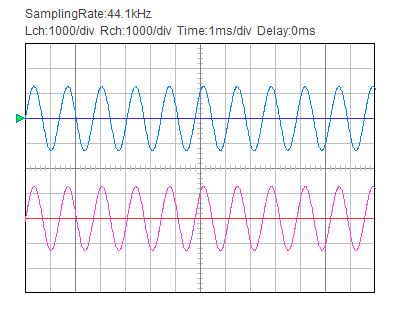
\includegraphics[width=0.45\linewidth]{result/day_4/osi_sine2}
  			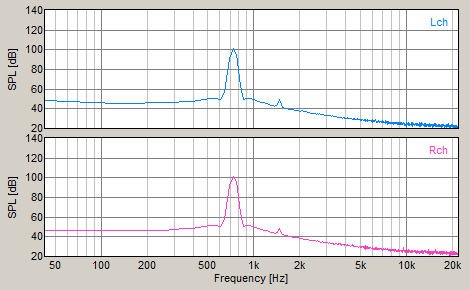
\includegraphics[width=0.45\linewidth]{result/day_4/fft_sine2}
  		\end{figure}

  		\item Skala 4 atau panjang buffer $512/4 = 128$.
  		Nilai frekuensi 1464 Hz dan nilai SPL 110 dB
  		\begin{figure}[H]
  			\centering
  			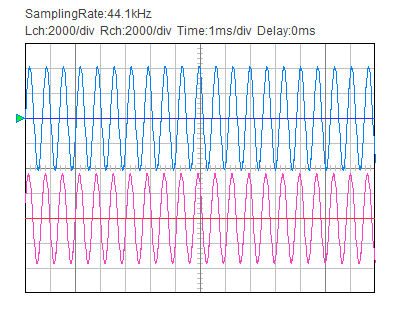
\includegraphics[width=0.45\linewidth]{result/day_4/osi_sine4}
  			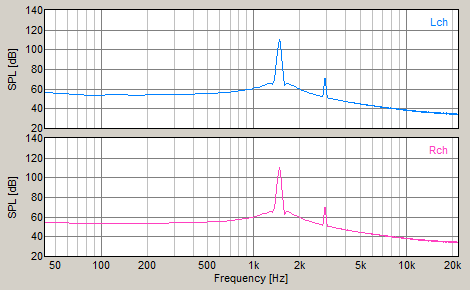
\includegraphics[width=0.45\linewidth]{result/day_4/fft_sine4}
  		\end{figure}

  		\item Skala 8 atau panjang buffer $512/8 = 64$.
  		Nilai frekuensi 2971 Hz dan nilai SPL 91 dB
  		\begin{figure}[H]
  			\centering
  			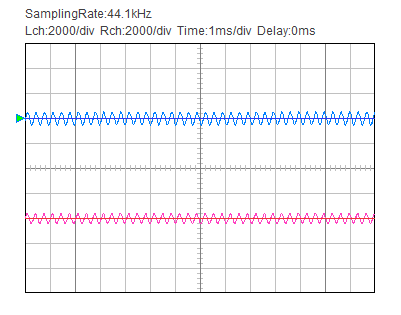
\includegraphics[width=0.45\linewidth]{result/day_4/osi_sine8}
  			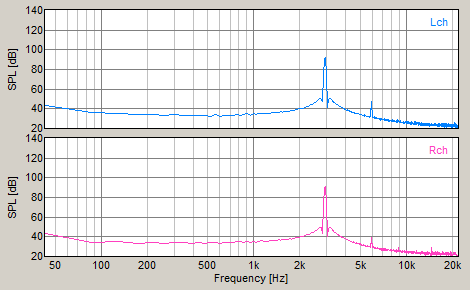
\includegraphics[width=0.45\linewidth]{result/day_4/fft_sine8}
  		\end{figure}

  		\newpage
  		\item Skala 16 atau panjang buffer $512/16 = 32$.
  		Nilai frekuensi 5900 Hz dan nilai SPL 90 dB
  		\begin{figure}[H]
  			\centering
  			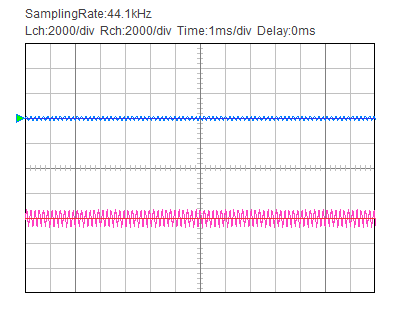
\includegraphics[width=0.45\linewidth]{result/day_4/osi_sine16}
  			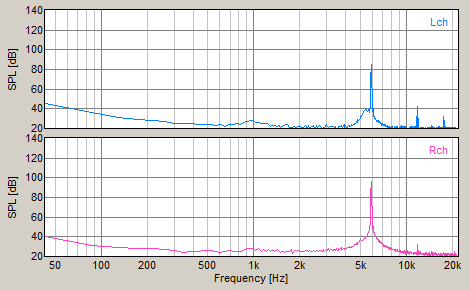
\includegraphics[width=0.45\linewidth]{result/day_4/fft_sine16}
  		\end{figure}

  		\item Skala 32 atau panjang buffer $512/32 = 16$.
  		Nilai frekuensi 11800 Hz dan nilai SPL 85 dB
  		\begin{figure}[H]
  			\centering
  			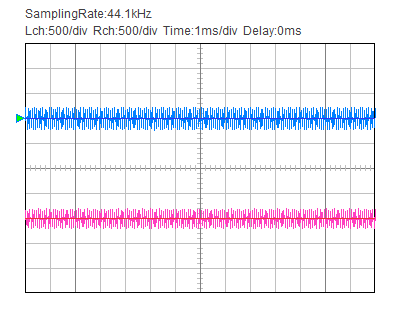
\includegraphics[width=0.45\linewidth]{result/day_4/newsinehighest}
  			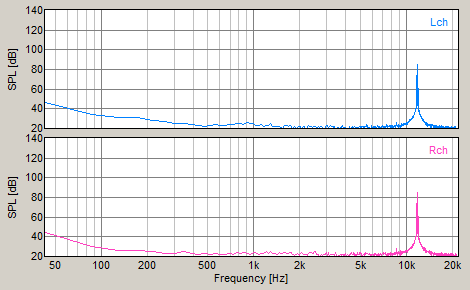
\includegraphics[width=0.45\linewidth]{result/day_4/newsinehighestfft}
  		\end{figure}

  		\item Skala 0.5 atau panjang buffer $512/0.5 = 1024$.
  		Nilai frekuensi 172 Hz dan nilai SPL 96 dB
  		\begin{figure}[H]
  			\centering
  			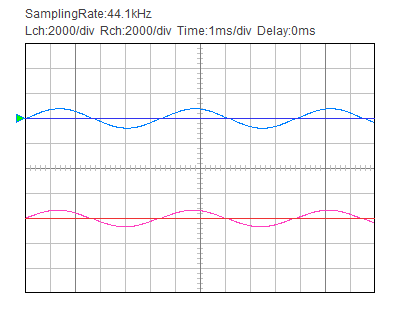
\includegraphics[width=0.45\linewidth]{result/day_4/osi_sine0p5}
  			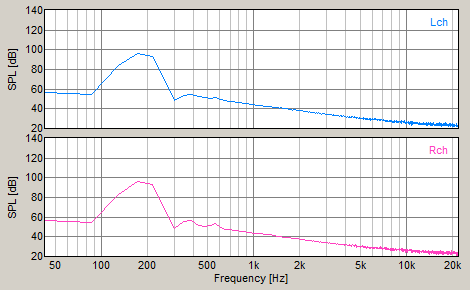
\includegraphics[width=0.45\linewidth]{result/day_4/fft_sine0p5}
  		\end{figure}

  		\newpage
  		\item Skala 0.25 atau panjang buffer $512/0.25 = 2048$.
  		Nilai frekuensi 86 Hz dan nilai SPL 92 dB
  		\begin{figure}[H]
  			\centering
  			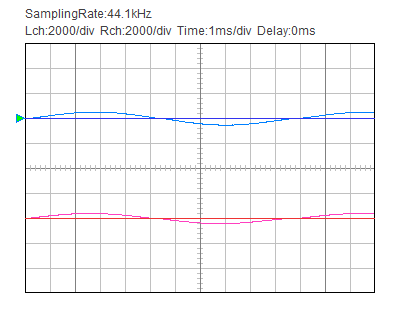
\includegraphics[width=0.45\linewidth]{result/day_4/osi_sine0p25}
  			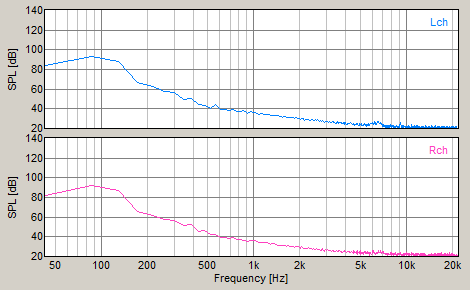
\includegraphics[width=0.45\linewidth]{result/day_4/fft_sine0p25}
  		\end{figure}
  	\end{itemize}

	Berikut plot hubungan antara skala frekuensi dengan frekuensi tone yang dihasilkan.
	Dengan diketahui hubungan skala dan frekuensi linear, maka model sine array dapat dimodifikasi dengan linear.
	\begin{figure}[H]
		\centering
		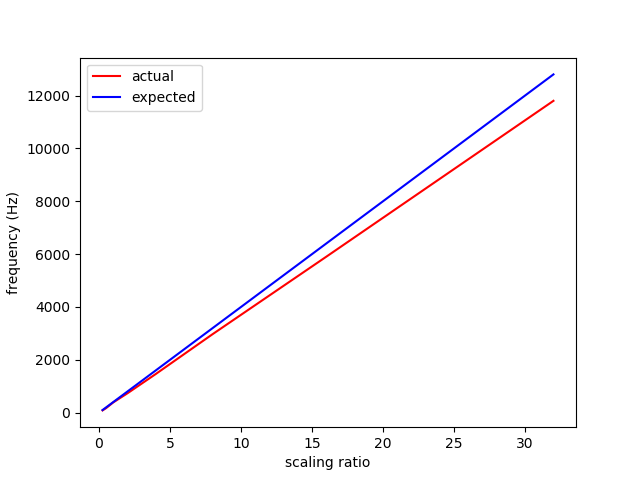
\includegraphics[width=0.45\linewidth]{result/analisa/freq_scaling}
	\end{figure}

	Dan berikut adalah hubungan	frekuensi dan SPL (\textit{Sound Pressure Level}) yang dihasilkan.
	Grafik sebelah kiri adalah hubungan frekuensi-SPL,
	sedangkan sebelah kanan adalah grafik respon frekuensi dari headphone.
	\begin{figure}[H]
		\centering
		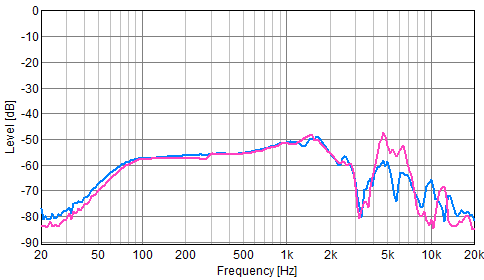
\includegraphics[width=0.45\linewidth]{result/day_1/FreqResp_JBL}
		\includegraphics[width=0.45\linewidth]{result/analisa/freq_spl}
	\end{figure}
	Dapat terlihat bahwa SPL tidak sepenuhnya konstan baik hasil \textit{frequency-response}
	maupun hasil modifikasi frekuensi pada amplitudo maksimal di setiap sinus array yang dihasilkan.

	\newpage
	\subsubsection{Pergeseran Amplitudo}
	Berikut adalah pengujian untuk modifikasi amplitudo dengan menggunakan model sinus yang sebelumnya.
	Amplitudo maksimal adalah 0.1 dari maksimal signed 16-bit ($0.1*32767=3277$).
	Kemudian amplitudo tersebut divariasi dengan skala 1 hingga 0.0001.
	Dengan pendekatan sangat kasar, jika 512 menghasilkan 400Hz (aktualnya 387 Hz), maka skala 1.25 atau $512/1.25=410$
	akan menghasilkan 500 Hz (aktualnya 473 Hz).
	Rangkuman model matematis:
	\[
	Y(i) =
	\begin{cases}
	S_A C_A sin(2 \pi \frac{i}{410}), \text{ if } Y \geq 0, \text{ for } 0 \leq i < 410\\
	S_A C_A sin(2 \pi \frac{i}{410})+65535, \text{ if } Y < 0, \text{ for } 0 \leq i < 410
	\end{cases}
	\]
	dengan $S_A$ adalah skala $1 \textasciitilde 0.0001$, dan $C_A=3277$ adalah konstanta amplitudo maksimal
	untuk signed 16-bit yang telah di atenuasi $0.1$.
	Model array-loop:
	\begin{minted}[frame=lines,fontsize=\footnotesize]{c}
double ampl;
buffsize = (uint16_t) 512/1.25;
for(i=0;i<buffsize;i++){
	ysin = ampl*0.1*32767*sin(2*3.141592653589793*((double)i/(double)buffsize));
	if(ysin >= 0){ i2s_tx_buf[i]=ysin; }
	if(ysin <0  ){ i2s_tx_buf[i]=ysin+65535; }
}
i2scfg.size = buffsize;
	\end{minted}

	Berikut hasil uji amplitudo untuk semua skala:
	\begin{itemize}
		\item Skala 1 dengan hasil amplitudo 98 dB.
		\begin{figure}[H]
			\centering
			\includegraphics[width=0.45\linewidth]{result/day_4/500Hz/tone1}
			\includegraphics[width=0.45\linewidth]{result/day_4/500Hz/fft_tone1}
		\end{figure}

		\item Skala 0.5 dengan hasil amplitudo 92 dB.
		\begin{figure}[H]
			\centering
			\includegraphics[width=0.45\linewidth]{result/day_4/500Hz/tone05}
			\includegraphics[width=0.45\linewidth]{result/day_4/500Hz/fft_tone05}
		\end{figure}

		\newpage
		\item Skala 0.1 dengan hasil amplitudo 72 dB.
		\begin{figure}[H]
			\centering
			\includegraphics[width=0.45\linewidth]{result/day_4/500Hz/tone01}
			\includegraphics[width=0.45\linewidth]{result/day_4/500Hz/fft_tone01}
		\end{figure}

		\item Skala 0.05 dengan hasil amplitudo 72 dB.
		\begin{figure}[H]
			\centering
			\includegraphics[width=0.45\linewidth]{result/day_4/500Hz/tone005}
			\includegraphics[width=0.45\linewidth]{result/day_4/500Hz/fft_tone005}
		\end{figure}

		\item Skala 0.01 dengan hasil amplitudo 58 dB.
		\begin{figure}[H]
			\centering
			\includegraphics[width=0.45\linewidth]{result/day_4/500Hz/tone001}
			\includegraphics[width=0.45\linewidth]{result/day_4/500Hz/fft_tone001}
		\end{figure}

		\newpage
		\item Skala 0.005 dengan hasil amplitudo 51 dB.
		\begin{figure}[H]
			\centering
			\includegraphics[width=0.45\linewidth]{result/day_4/500Hz/tone0005}
			\includegraphics[width=0.45\linewidth]{result/day_4/500Hz/fft_tone0005}
		\end{figure}

		\item Skala 0.001 dengan hasil amplitudo 42 dB.
		\begin{figure}[H]
			\centering
			\includegraphics[width=0.45\linewidth]{result/day_4/500Hz/tone0001}
			\includegraphics[width=0.45\linewidth]{result/day_4/500Hz/fft_tone0001}
		\end{figure}

		\item Skala 0.0005 dengan hasil amplitudo 47 dB.
		\begin{figure}[H]
			\centering
			\includegraphics[width=0.45\linewidth]{result/day_4/500Hz/tone00005}
			\includegraphics[width=0.45\linewidth]{result/day_4/500Hz/fft_tone00005}
		\end{figure}

		\newpage
		\item Skala 0.0001 dengan hasil amplitudo 42 dB.
		\begin{figure}[H]
			\centering
			\includegraphics[width=0.45\linewidth]{result/day_4/500Hz/tone00001}
			\includegraphics[width=0.45\linewidth]{result/day_4/500Hz/fft_tone00001}
		\end{figure}
	\end{itemize}

	Kemudian berikut hasil plot logaritmic dari skala amplitudo dengan aktual amplitudo.
	\begin{figure}[H]
		\centering
		\includegraphics[width=0.75\linewidth]{result/analisa/ampl_scaling}
	\end{figure}
	Maka terlihat untuk skala logaritma bersesuian dengan skala logaritma amplitudo.

	\newpage
	\section{Rangkuman}

	\subsection{Pencapaian}
	Beberapa poin pencapaian yang dapat dirangkum:
	\begin{enumerate}
		\item Model sinus yang paling bersih adalah sebagai berikut:
		\begin{itemize}
			\item Matematis:
			\[ B = 512/F \]
			\[
			Y(i) =
			\begin{cases}
			A sin(2 \pi \frac{i}{B}), \text{ if } Y \geq 0, \text{ for } 0 \leq i < B\\
			A sin(2 \pi \frac{i}{B})+65535, \text{ if } Y < 0, \text{ for } 0 \leq i < B
			\end{cases}
			\]
			dengan A adalah nilai maksimal variabel \textit{signed 16-bit} yaitu 32767
			dan F adalah skala untuk memodifikasi panjang array buffer.

			\item Array-Loop pada clock I2S dan Sampling BCLK adalah 16kHz:
			\begin{minted}[frame=lines,fontsize=\footnotesize]{c}

double ampl;
uint16_t buffsize = (uint16_t) 512/freq;
for(i=0;i<buffsize;i++){
	ysin = 0.1*32767*ampl*sin(2*3.141592653589793*((double)i/(double)buffsize));
	if(ysin >= 0){ i2s_tx_buf[i]=ysin; }
	if(ysin <0  ){ i2s_tx_buf[i]=ysin+65535; }
}
i2scfg.size = buffsize;
			\end{minted}
		\end{itemize}

		\item Frekuensi dan panjang array buffer adalah \textbf{Linear}.

		\item Respon logaritmik amplitudo dan SPL adalah \textbf{Linear}.
	\end{enumerate}

	\subsection{Belum Terselesaikan}
	Berikut beberapa poin yang belum terselesaikan dapat dirangkum:
	\begin{itemize}
		\item Kompensasi headphone yang memiliki respon amplitudo yang
		tidak flat (datar/konstan) terhadap frekuensi.

		\item Perbedaan signifikan antara array untuk PCM mono dan array PCM stereo.

		\item Masalah \text{Audio POP} yang masih muncul di akhir \textit{tone play}.
	\end{itemize}

	Pengembangan selanjutnya membutuhkan instrumen \textit{Audio Capture/Analyzer}
	walaupun tidak mengharuskan menggunakan manekin KEMAR.

\end{document}
